% Chapter Template

\chapter{Introduction} 
\label{chapter-1} 

%----------------------------------------------------------------------------------------
%	SECTION 
%----------------------------------------------------------------------------------------

\section{Motivation}

\begin{itemize}
\item AI -- DL -- lots of applications/advances/succes-stories in recent years perception (not reasoning yet). Cite important papers/reviews and exciting applications (autonomous driving, \ldots)
\item Cite/explain two multimodal examples: heart disease from multiple sensors and lip/audio speech recognition. This is multimodal (more general than multisensorial, more on this in Section Background)
\item Common good practice in engineering is if one sensor/process fails, other will take over (name for this?). Humans cocktail-party effect, cross-modal attention.
\item Most AI systems are tested in ideal situations, not realistic. Imagine when one sensor fails, or noisy or unknown (outlying).. AI systems are not explicitly prepared for this.
\item I introduce EMMA that solves previous paragraph problem
\item What this thesis is about
\end{itemize}
\href{http://www.scholarpedia.org/article/Crossmodal_attention}{crossmodal attention}

%----------------------------------------------------------------------------------------
%	SECTION 
%----------------------------------------------------------------------------------------

\section{Proposed solution}

Introduce model + modes + prediction. We will only see DL models because better at perception.

\begin{figure}[!h]
\centering
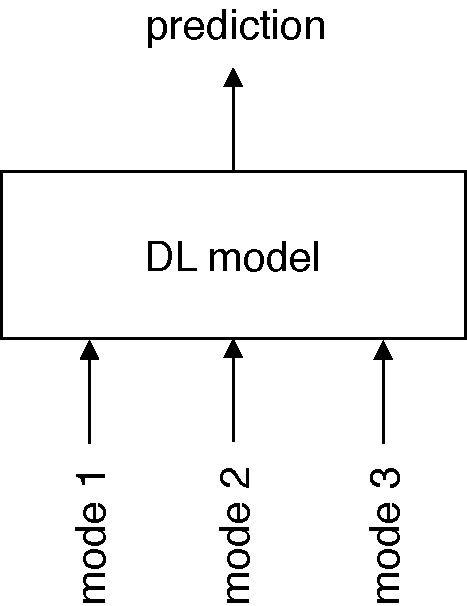
\includegraphics[scale=0.5]{figures/introduction-three-modes}
\caption{Main idea}	
\label{fig:main-idea}
\end{figure}

Problem is when outlying -- possibly high activations -- drop in performances (more on this in next chapter). Principle of solution (loosily inspired by dropout) is quiet simple (oversimplified on purpose): outlying is multiplied by small number close/greater to zero, other by number close/less to 1 (unchanged). Explain diagram only test-time (not speaking about training).
\begin{figure}[!h]
\centering
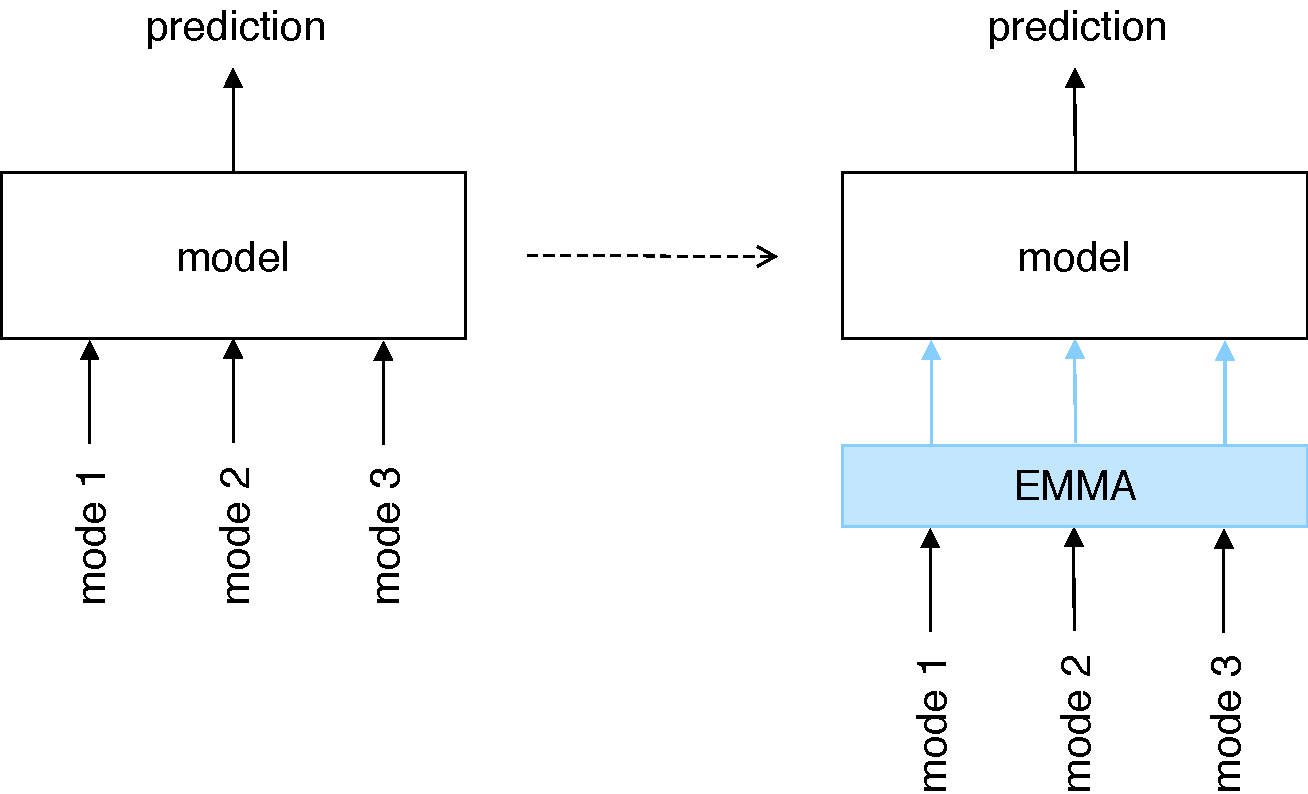
\includegraphics[scale=0.5]{figures/introduction-three-modes-with-emma}
\caption{Main idea}	
\label{fig:main-idea}
\end{figure}


%----------------------------------------------------------------------------------------
%	SECTION 
%----------------------------------------------------------------------------------------

\section{Thesis Outline}

High level overview of this work. Contributions.